\documentclass[10pt,a4paper,landscape, hidelinks]{article}
\usepackage{multicol}
\usepackage{calc}
\usepackage{ifthen}
\usepackage[footskip=.6cm,landscape]{geometry}
\usepackage{hyperref}
\usepackage{enumitem}
\usepackage{amsmath}
\usepackage{amssymb}
\usepackage{stix}
\usepackage{tabto}
\usepackage{scalerel}
\usepackage[utf8]{inputenc}
\usepackage[T1]{fontenc}
\usepackage[ngerman]{babel}
\usepackage{graphicx}

\graphicspath{{./bilder/}}

% To make this come out properly in landscape mode, do one of the following
% 1.
%  pdflatex latexsheet.tex
%
% 2.
%  latex latexsheet.tex
%  dvips -P pdf  -t landscape latexsheet.dvi
%  ps2pdf latexsheet.ps


% If you're reading this, be prepared for confusion.  Making this was
% a learning experience for me, and it shows.  Much of the placement
% was hacked in; if you make it better, let me know...


% 2008-04
% Changed page margin code to use the geometry package. Also added code for
% conditional page margins, depending on paper size. Thanks to Uwe Ziegenhagen
% for the suggestions.

% 2006-08
% Made changes based on suggestions from Gene Cooperman. <gene at ccs.neu.edu>


% To Do:
% \listoffigures \listoftables
% \setcounter{secnumdepth}{0}


% This sets page margins to .5 inch if using letter paper, and to 1cm
% if using A4 paper. (This probably isn't strictly necessary.)
% If using another size paper, use default 1cm margins.
\ifthenelse{\lengthtest { \paperwidth = 11in}}
	{ \geometry{top=.5in,left=.5in,right=.5in,bottom=.5in} }
	{\ifthenelse{ \lengthtest{ \paperwidth = 297mm}}
		{\geometry{top=.5cm,left=0.8cm,right=0.8cm,bottom=1cm} }
		{\geometry{top=1cm,left=1cm,right=1cm,bottom=1cm} }
	}

% Turn off header and footer
\pagestyle{plain}
%\pagenumbering{arabic}


% Redefine section commands to use less space
\makeatletter
\renewcommand{\section}{\@startsection{section}{1}{0mm}%
                                {-1ex plus -.5ex minus -.2ex}%
                                {0.5ex plus .2ex}%x
                                {\normalfont\large\bfseries}}
\renewcommand{\subsection}{\@startsection{subsection}{2}{0mm}%
                                {-1explus -.5ex minus -.2ex}%
                                {0.5ex plus .2ex}%
                                {\normalfont\normalsize\bfseries}}
\renewcommand{\subsubsection}{\@startsection{subsubsection}{3}{0mm}%
                                {-1ex plus -.5ex minus -.2ex}%
                                {1ex plus .2ex}%
                                {\normalfont\small\bfseries}}
\makeatother
\newcommand*\variant[1]{\bar{#1}}

% Define BibTeX command
\def\BibTeX{{\rm B\kern-.05em{\sc i\kern-.025em b}\kern-.08em
    T\kern-.1667em\lower.7ex\hbox{E}\kern-.125emX}}

% Don't print section numbers
%\setcounter{secnumdepth}{0}


\setlength{\parindent}{0pt}
\setlength{\parskip}{0pt plus 0.5ex}


% -----------------------------------------------------------------------

\begin{document}

\raggedright
\footnotesize
\begin{multicols*}{3}


% multicol parameters
% These lengths are set only within the two main columns
%\setlength{\columnseprule}{0.25pt}
\setlength{\premulticols}{1pt}
\setlength{\postmulticols}{1pt}
\setlength{\multicolsep}{1pt}
\setlength{\columnsep}{2pt}

% page for TOC
% exclude from numbering
\thispagestyle{empty}
\tableofcontents
\newpage
\pagenumbering{arabic}

\begin{center}
     \Large{\textbf{TMB Formelsammlung}} \\
\end{center}

\section{Statik}

\subsection{Grundgleichungen der Statik}
\tabto{0.35cm}$\sum{F_x}=0\qquad\sum{F_y}=0\qquad\sum{M^P}=0$

\subsection{Trigonometrische Sätze}
\begin{itemize}[leftmargin=*]
        \item[] Sinussatz\tabto{2cm} $\frac{a}{\sin(\alpha)}=\frac{b}{\sin(\beta)}=\frac{c}{\sin(\gamma)}$
        \item[] Kosinussatz\tabto{2cm} $c^2=a^2+b^2-2\cdot a\cdot b\cdot\cos(\gamma)$
        \item[] Summensätze\tabto{2cm} $\sin(\alpha)\cdot\cos(\alpha)=\sin(2\cdot\alpha)$
        \item[] \tabto{2cm} $\sin(\alpha+\beta)=\sin(\alpha)\cdot\cos(\beta)+\sin(\beta)\cdot\cos(\alpha)$
        \item[] \tabto{2cm} $\cos(\alpha+\beta)=\cos(\alpha)\cdot\cos(\beta)-\sin(\beta)\cdot\sin(\alpha)$
\end{itemize}

\subsection{Standsicherheit}
\begin{itemize}[leftmargin=*]
        \item [] $\sum M_{Stand}=s_f\cdot\sum M_{Kipp}$
        \tabto{4cm}{\scriptsize$s_f$ ...Sicherheit gegen Kippen}
\end{itemize}

\subsection{Reibung}
\begin{itemize}[leftmargin=*]
        \item[] Haftreibung\tabto{2cm} $F_{R_{max}}=F_N\cdot\mu$\tabto{4.5cm}{\scriptsize wenn $v=0$, $F_R$ aus\\
                                                                \tabto{4.5cm}Gleichgewichtsbedingungen}
        \item[] Gleitreibung\tabto{2cm} $F_R=F_N\cdot\mu$
        \item[] Seilreibung\tabto{2cm} $F_z\le F_h\cdot e^{\mu\cdot\alpha}$\tabto{4.5cm}{\scriptsize$\alpha$ ...Winkel in $rad$}\\
\end{itemize}


\section{Festigkeitslehre}
\begin{itemize}[leftmargin=*]
        \item [] Flächenschwerpunkt\tabto{3cm} $x_S=\frac{\sum x_i\cdot A_i}{\sum A_i}=\frac{1}{A}\cdot\int x\cdot dA $
\end{itemize}

\subsection{Flächenmomente und Deviationsmomente}
\begin{itemize}[leftmargin=*]
        \item [] Flächenmomente\tabto{2.7cm} $I_y=\int z^2\cdot dA$\\
        \tabto{2.7cm}$I_z=\int y^2\cdot dA$
        \item [] Deviationsmomente\tabto{2.7cm} $I_{yz}=\int y\cdot z\cdot dA$\\
        \tabto{2.7cm}{\scriptsize negatives Vorzeichen in SE}
        \item [] polares Widerstandsmoment\tabto{4cm} $I_p=I_x+I_y$
\end{itemize}

\subsection{Satz von Steiner}
\begin{itemize}[leftmargin=*]
        \item [] $I_y^P=I_y^S+A\cdot y^2$\makebox[1.36cm]{\hfill}$I_y^S=I_y^P-A\cdot y^2$
        \item [] $I_{yz}^P=I_{yz}^S-A\cdot y\cdot z$\makebox[1cm]{\hfill}$I_{yz}^S=I_{yz}^P+A\cdot y\cdot z$
        \item [] {\scriptsize festlegen:$\quad\Delta{y}=y_{S_\text{einzel}}-y_{S_\text{ges}}$}
\end{itemize}

\subsection{Normalspannungen}

\subsubsection{Zug und Druck}
\tabto{0.35cm}$\sigma_\text{Z/D}=\frac{F_\text{Z/D}}{A}=E\cdot\epsilon=E\cdot\frac{\Delta l}{l_0}$
\subsubsection{Biegung}
\tabto{0.35cm}$\sigma_B=\frac{M_B}{W_B}=\frac{M_B}{I}\cdot z$\tabto{3.5cm}{\scriptsize$z$ ...Schwerpunktabstand}
\subsubsection{Flächenträgheitsmomente}
\begin{itemize}[leftmargin=*]
        \item [] Rechteck\tabto{2cm} $I_{x_\square}=\frac{h^3\cdot b}{12}$
        \item [] Kreis\tabto{2cm} $I_{x_\circ}=\frac{d^4\cdot\pi}{64}$
        \item [] Kreisring\tabto{2cm} $I_\text{KR}=\frac{(D^4-d^4)\cdot\pi}{64}$
        \item [] Dreieck\tabto{2cm} $I_{x_\lrtriangle}=\frac{b\cdot h^3}{36}$\tabto{3.7cm}$I_{xy_\lrtriangle}=\frac{b^2\cdot h^2}{72}$
\end{itemize}

\subsubsection{Schnittgrößen}
\tabto{0.35cm}$Q(x_i)=Q_0\pm\int_0^{x_i}{q(x)\cdot dx}$\tabto{4.5cm}$Q(x_{M_\text{max}})=0\quad\longrightarrow\quad x_{M_\text{max}}$
\tabto{0.35cm}$M(x_i)=M_0\mp\int_0^{x_i}{Q(x)\cdot dx}$\tabto{4.5cm}$M_\text{max}=M(x_{M_\text{max}})$
\tabto{0.35cm}$M_\text{Streckenl.}(x_i)=\int_{0}^{x_i}{q(x)\cdot x\cdot dx}$

\columnbreak
%---------------------------------------------------------------------------

\subsubsection{Schiefe Biegung}
Drehung des Kooridnatsystems um den Schwepunkt:
\begin{itemize}[leftmargin=*]
        \item [] $I_\eta=\frac{I_y+I_z}{2}+\frac{I_y-I_z}{2}\cdot\cos(2\cdot\phi)+I_{yz}\cdot\sin(2\cdot\phi)$
        \item [] $I_\zeta=\frac{I_y+I_z}{2}+\frac{I_y-I_z}{2}\cdot\cos(2\cdot\phi)-I_{yz}\cdot\sin(2\cdot\phi)$
        \item [] $I_{\eta\zeta}=-\frac{I_y-I_z}{2}\cdot\sin(2\cdot\phi)+I_{yz}\cdot\cos(2\phi)$
\end{itemize}
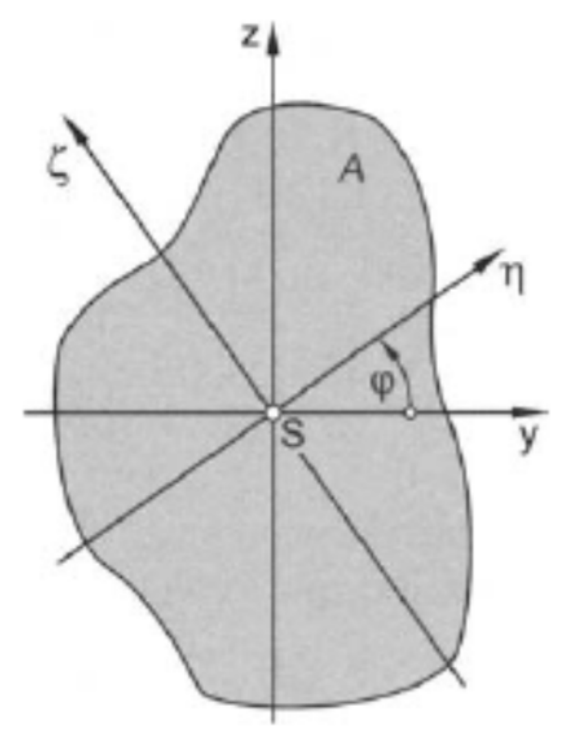
\includegraphics[width=2cm]{2-3-5_Drehung-des-Koordinatensystems}

Richtungswinkel gegen den Uhrzeigersinn:
\begin{itemize}[leftmargin=*]
        \item [] $\phi_{1;2}=\frac{1}{2}\cdot\arctan\left(\frac{2\cdot I_{yz}}{I_y-I_z}\right)$
        \begin{math}
                -2\cdot(I_y-I_z)\cdot\cos(2\cdot\phi)-4\cdot I_{yz}\cdot\sin(2\cdot\phi)
                \begin{cases}
                        <0\rightarrow\text{Hauptachse}\\
                        \ge0\rightarrow\text{Nebenachse}\\
                \end{cases}
        \end{math}
\end{itemize}

Maximales Flächenmoment:
\begin{itemize}[leftmargin=*]
        \item [] $I_{HA}=I_1=\frac{I_y+I_z}{2}+\sqrt{\left(\frac{I_y-I_z}{2}\right)^2+I_{yz}^2}$
\end{itemize}

Minimales Flächenmoment:
\begin{itemize}[leftmargin=*]
        \item [] $I_{NA}=I_2=\frac{I_y+I_z}{2}-\sqrt{\left(\frac{I_y-I_z}{2}\right)^2+I_{yz}^2}$
\end{itemize}

Abstandsabhängige Gesamt-Normalspannung:
\begin{itemize}[leftmargin=*]
        \item [] $\sigma(y_{HA},z_{HA})=\pm\frac{M_{HA}}{I_1}\cdot z_{HA}\pm\frac{M_{NA}}{I_2}\cdot y_{HA}\pm\frac{F_{Z/D}}{A}$
        \item [] $\sigma_x(y,z)=\frac{M_y}{I_{yy}}\cdot z-\frac{M_z}{I_{zz}}\cdot y\pm\frac{F_{Z/D}}{A}$
\end{itemize}

Normalspannung Nullinie:
\begin{itemize}[leftmargin=*]
        \item [] $\sigma_x(y,z)=0\quad\longrightarrow\quad y(z)\quad\text{oder}\quad z(y)$
\end{itemize}

\subsubsection{Knickung}
Knickung nach Euler:\\
\includegraphics[width=7cm]{2-3-6_Knickfälle}
\begin{itemize}[leftmargin=*]
        \item [] $F_K=\frac{\pi^2\cdot E\cdot I}{L_K^2}\qquad\qquad$ Knicksicherheit $S=\frac{F_K}{F}$\\
        \item [] $\sigma_K=\frac{F_k}{A}=\frac{\pi^2\cdot E\cdot I}{L_K^2\cdot A}=\frac{\pi^2\cdot E}{\lambda^2}$\\
        \item []
        \begin{math}
                \lambda_G=\sqrt{\pi\cdot\frac{E}{\sigma_{DB}}}\qquad\sigma_{DB}=\sigma\newline
                \lambda=\sqrt{\frac{L_K^2\cdot A}{I}}=
                \begin{cases}
                        \text{\scriptsize ...Schlankheitsgrad}\\
                        >90\textsl{ bzw.} >\lambda_g\rightarrow\text{Euler}\\
                        \text{ansonsten}\rightarrow\text{Tetmajr oder Quetschen (Zug/Druck)}
                \end{cases}
        \end{math}
\end{itemize}

\columnbreak
%---------------------------------------------------------------------------

Knickung nach Tetmajr:\\
\tabto{0.35cm}$\sigma_K=a-b\cdot\lambda+c\cdot\lambda^2$\tabto{3.5cm}{\scriptsize(a, b, c aus Tabelle)}
%[!]TODO: aus welcher Tabelle?

\subsection{Querspannungen}

\subsubsection{Abscherung}
\tabto{0.35cm}$\tau_A=\frac{F_Q}{A}$

\subsubsection{Schub infolge Querkraft}
\begin{itemize}[leftmargin=*]
        \item [] $\tau_S=\frac{F_Q\cdot s_x}{I^{S_\text{ges}}_x\cdot b(z)}\qquad\qquad\tau_\text{max}=\frac{4}{3}\cdot\tau_\text{mittel}$
        \item [] $s_x=A_{\text{Rest}}\cdot z_{\text{Rest}}$
        \item [] $F_N=\tau_s\cdot b(z)\cdot l_N$
\end{itemize}
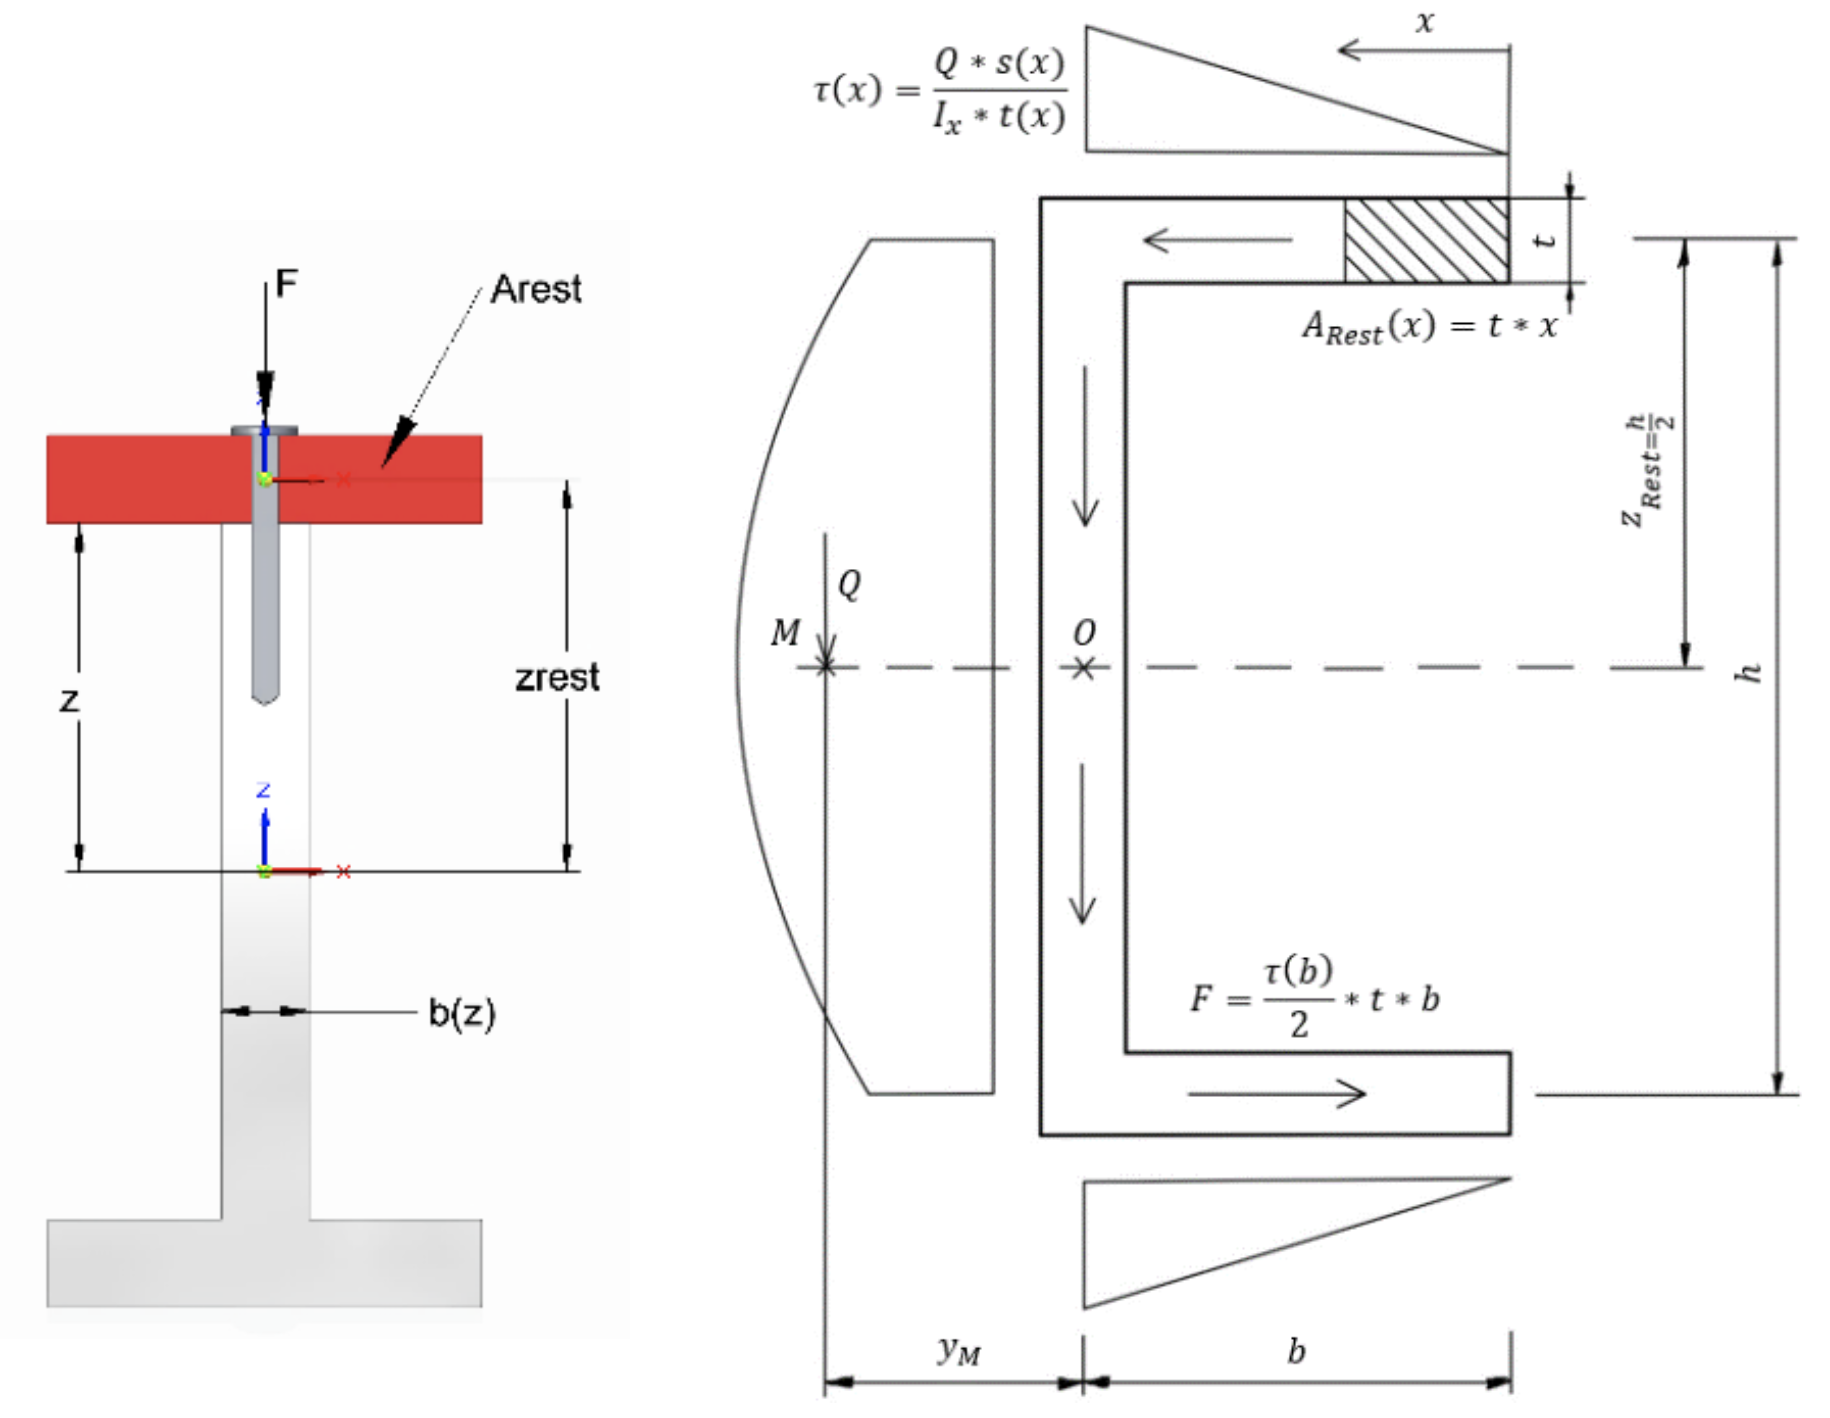
\includegraphics[width=5cm]{2-4_Schub-infolge-Querkraft}

\subsubsection{Torsion}
\begin{itemize}[leftmargin=*]
        \item [] $\tau_T=\frac{M_T}{W_T}=\frac{M_T}{I_p}\cdot z$\tabto{3.5cm}{\scriptsize$z$ ...Schwerpunktabstand}
        \item [] $\phi=\frac{M_T\cdot l}{G\cdot I_p}\qquad\qquad[\phi]=rad$
\end{itemize}
polare Flächenträgheitsmomente und Widerstandsmomente:
\begin{itemize}[leftmargin=*]
        \item [] Kreis\tabto{1.5cm}$I_{p_\circ}=\frac{d^4\cdot\pi}{32}$\tabto{4cm}$W_{T_\circ}=\frac{d^3\cdot\pi}{16}$
        \item [] Kreisring\tabto{1.5cm}$I_{p_\text{KR}}=\frac{(D^4-d^4)\cdot\pi}{32}$\tabto{4cm}$W_{T_\circ}=\frac{(D^4-d^4)\cdot\pi}{16\cdot D}$
\end{itemize}

\subsection{Wärmedehnung}
\tabto{0.35cm}$\Delta{l}=\alpha\cdot l_0\cdot\Delta{T}$

\subsection{Flächenpressung}
\tabto{0.35cm}$p=\frac{F}{A_\text{proj.}}$

\subsection{Vergleichsspannungen}
\begin{itemize}[leftmargin=*]
        \item [] $\tau=\tau\cdot\alpha_0$\tabto{2cm}$\alpha_0=\frac{\sigma_\text{zul.}}{\eta\cdot\tau_\text{zul.}}$\tabto{4cm}$\sigma=\sigma_b\pm\sigma_\text{Z/D}$
        \item [] Normalspannungshypothese ($\eta=1$):\\
        $\sigma_v=\frac{\sigma}{2}+\sqrt{\left(\frac{\sigma}{2}\right)^2+\tau^2}$
        \item [] Schubspannungshypothese ($\eta=2$):\\
        $\sigma_v=\sqrt{\sigma^2+4\cdot \tau^2}$
        \item [] Gestaltänderungsenergiehypothese GEH $\left(\eta=\sqrt{3}\right)$:\\
        $\sigma_v=\sqrt{\sigma^2+3\cdot \tau^2}$
\end{itemize}

\columnbreak
%---------------------------------------------------------------------------

\subsection{Biegelinie}
\begin{itemize}[leftmargin=*]
        \item [] $W''(x)=-\frac{M(x)}{E\cdot I}$
        \item [] $W'(x)=\int{W''(x)}+c_1$
        \item [] $W(x)=\int{W'(x)}+c_2=\int{W''(x)}+c_1\cdot x+c_2$
        \item [] {\scriptsize Variablen/-anzahl und Gleichungen/-anzahl Dokumentieren}
\end{itemize}
\includegraphics[width=9cm]{2-8_Biegelinie-Krümmung-Vorzeichen}

\subsection{Satz von Castigliano}
\begin{itemize}[leftmargin=*]
        \item [] $y=\frac{\partial{W}}{\partial{F}}\qquad F=\frac{\partial{W}}{\partial{y}}\qquad \phi=\frac{\partial{W}}{\partial{M}}\qquad M=\frac{\partial{W}}{\partial{\phi}}$\\ \\
        \item [] $y=\displaystyle{\sum_i{\int_{0}^{l_i}}}{\frac{N_i(x_i)}{E_i\cdot A_i}\cdot \frac{\partial{N_i(x_i)}}{\partial{F}}}\cdot dx_i$
                $+\displaystyle{\sum_i{\int_{0}^{l_i}}}{\frac{M_{B_i}(x_i)}{E_i\cdot I_i}\cdot \frac{\partial{M_{B_i}(x_i)}}{\partial{F}}}\cdot dx_i$\\ \\
                $\quad+\displaystyle{\sum_i{\int_{0}^{l_i}}}{\frac{M_{T_i}(x_i)}{G_i\cdot I_{p_i}}\cdot \frac{\partial{M_{T_i}(x_i)}}{\partial{F}}}\cdot dx_i$\\ \\ \\
        \item [] $\phi=\displaystyle{\sum_i{\int_{0}^{l_i}}}{\frac{M_{B_i}(x_i)}{E_i\cdot I_i}\cdot \frac{\partial{M_{B_i}(x_i)}}{\partial{M}}}\cdot dx_i+
                \displaystyle{\sum_i{\int_{0}^{l_i}}}{\frac{M_{T_i}(x_i)}{G\cdot I_{p_i}}\cdot \frac{\partial{M_{T_i}(x_i)}}{\partial{M}}}\cdot dx_i$
\end{itemize}
\subsubsection{Satz von Menabrea}
\begin{itemize}[leftmargin=*]
        \item [] Fest-/Loslager $F_\text{Lager}$:\tabto{3.2cm}$y=0\quad\longrightarrow\quad F_\text{Lager}$
        \item [] Einspannstelle $M_\text{Einsp.}$:\tabto{3.2cm}$\phi=0\quad\longrightarrow\quad M_\text{Einsp.}$
\end{itemize}

\section{Hydromechanik}
\subsection{Kräfte}
\begin{itemize}[leftmargin=*]
        \item [] $F_\text{Druck}=p_{ges}\cdot A_{proj.}$
        \item [] $p_{stat}=p_0+\rho\cdot g\cdot h$\tabto{3.3cm}$\left[p_{stat}\right]=\text{Pa}$
        \item [] $F_\text{Auftr.}=\rho_\text{Fl.}\cdot g\cdot V_\text{verdr.}$\tabto{3.3cm}...Vertikalkompnente (durch Schwp.)
        \item [] $F_\text{H}=\rho\cdot g\cdot h_S\cdot A_\text{proj.}$\tabto{3.3cm}...Horizontalkomponente
\end{itemize}

\subsection{Druckmittelpunkt}
\begin{itemize}[leftmargin=*]
        \item [] $y_{SD}=y_D-y_S=\frac{I_x^S}{A\cdot y_S}\qquad\qquad x_D=x_S$
\end{itemize}
\includegraphics[width=6cm]{3-2_Hydromechanik-Kräfte}


\columnbreak
%---------------------------------------------------------------------------

\subsection{Bernoulli-Gleichung – Energieerhaltung}
\begin{itemize}[leftmargin=*]
        \item [] $\dot{m}=\rho\cdot\dot{V}=\rho\cdot A\cdot v$
        \item [] \textbf{Druckform:}\\
        $\rho\cdot g\cdot h_1+\rho\cdot\frac{v_1^2}{2}+p_1+\frac{P_\text{P}\cdot\rho}{\dot{m}}=\rho\cdot g\cdot h_2+\rho\cdot\frac{v_2^2}{2}+p_2+p_\text{VE}$
        \item [] \textbf{Höhenform:}\\
        $h_1+\frac{v_1^2}{2\cdot g}+\frac{p_1}{\rho\cdot g}+\frac{P_\text{P}}{\dot{m}\cdot g}=h_2+\frac{v_2^2}{2\cdot g}+\frac{p_2}{\rho\cdot g}+h_\text{VE}$
\end{itemize}

\subsection{Strömungsverluste \& Moody-Diagramm}
\begin{itemize}[leftmargin=*]
        \item [] \textbf{örtliche Verluste:}
        \item [] $h_\text{VE}=\zeta\cdot\frac{v^2}{2\cdot g}$
        \item [] \textbf{Streckenverluste:}
        \item [] $h_\text{VS}=\lambda\cdot\frac{l}{d_\text{hydr.}}\cdot\frac{v^2}{2\cdot g}$
        \item [] $d_\text{hydr.}=\frac{4\cdot A}{U_\text{benetzt}}$
        \item [] $Re=\frac{v\cdot d_\text{hydr.}}{v_K}$\tabto{3cm}$v_K$ ...kinetische Zähigkeit ($v_{\text{H}_2\text{O}}=10^{-6}\frac{\text{m}^2}{\text{s}}$)
\end{itemize}

\subsection{Impulserhaltung und Stützkräfte}
\begin{itemize}[leftmargin=*]
        \item [] $|S|=p_{"u}\cdot A+\dot{m}\cdot v$\tabto{3cm}$S$ ...Stützkraft
\end{itemize}

\section{Thermodynamik}
\subsection{ideales Gas}
\begin{itemize}[leftmargin=*]
        \item [] $p\cdot V=m\cdot R\cdot T\qquad\qquad p\cdot v=R\cdot T$
        \item [] $R=\frac{8314}{M}\qquad\left[R\right]=\frac{\text{J}}{\text{kg}\cdot\text{K}}$
        \item [] $\kappa=\frac{c_p}{c_v}\qquad R=c_p-c_v$
        \item [] $\quad\Rightarrow\quad c_v=\frac{R}{\kappa-1}\qquad c_p=\frac{R\cdot\kappa}{\kappa-1}$
\end{itemize}

\subsection{Hauptsätze der Thermodynamik}
\begin{itemize}[leftmargin=*]
        \item [] 1. Hauptsatz der Thermodynamik:\\
                $dQ+dA=(dEa)+dU$
        \item [] 2. Hauptsatz der Thermodynamik:\\
                $ds=\frac{dq}{T}$
        \item [] Arbeit - geschlossenes System:\\
                $A_v=-\int_{1}^{2}{p\cdot dV}$
        \item [] Arbeit - offenes System:\\
                $A_t=\int_{1}^{2}{V\cdot dp=H_2-H_1-Q_a}$
        \item [] Wärme:\\
                $dQ=dU+p\cdot dV=dH-V\cdot dp$\tabto{5cm}
                $h=u+p\cdot v$
\end{itemize}

\columnbreak
%---------------------------------------------------------------------------

\subsection{Zustandsänderungen ideales Gas}
\includegraphics[width=6cm]{4-3_Zustandsänderungen}
\begin{itemize}[leftmargin=*]
        \item [] \textbf{Isochor:} \fbox{$V_1=V_2$} $\qquad n=\infty$
        \subitem $\frac{p_1}{p_2}=\frac{T_1}{T_2}$
        \subitem $q_{12}=u_{12}=c_v\cdot(T_2-T_1)$
        \subitem $a_t=R\cdot(T_2-T_1)=v\cdot(p_2-p_1)$
        \subitem $a_v=0$
        \subitem $s_{12}=c_v\cdot\ln{\left(\frac{T_2}{T_1}\right)}$
        \item [] \textbf{Isobar:} \fbox{$p_1=p_2$} $\qquad n=0$
        \subitem $\frac{V_1}{V_2}=\frac{v_1}{v_2}=\frac{T_1}{T_2}$
        \subitem $q_{12}=h_{12}=c_p\cdot(T_2-T_1)\qquad\rightarrow\text{für Dampf: }q_{12}=h_{12}$
        \subitem $a_t=0$
        \subitem $a_v=-R\cdot(T_2-T_1)=-p\cdot(v_2-v_1)$
        \subitem $s_{12}=c_p\cdot\ln{\left(\frac{T_2}{T_1}\right)}$
        \item [] \textbf{Isotherm/Isenthalp:} \fbox{$T_1=T_2$}$\quad$\&$\quad$\fbox{$h_{12}=0$} $\qquad n=1$
        \subitem $\frac{p_1}{p_2}=\frac{v_2}{v_1}=\frac{V_2}{V_1}$
        \subitem $q_{12}=R\cdot T\cdot\ln{\left(\frac{p_1}{p_2}\right)}=-R\cdot T\cdot\ln{\left(\frac{v_1}{v_2}\right)}$
        \subitem $a_t=a_v=-q_{12}=-R\cdot T\cdot\ln{\left(\frac{p_1}{p_2}\right)}=R\cdot T\cdot\ln{\left(\frac{v_1}{v_2}\right)}$
        \subitem $a_v=a_t=-q_{12}=-R\cdot T\cdot\ln{\left(\frac{p_1}{p_2}\right)}=R\cdot T\cdot\ln{\left(\frac{v_1}{v_2}\right)}$
        \subitem $s_{12}=R\cdot\ln{\left(\frac{p_1}{p_2}\right)}$
        \item [] \textbf{Isentrop:} \fbox{$S_1=S_2$}$\qquad n=\kappa\quad${\scriptsize(adiabat \& reibungsfrei)}
        \subitem $p_1\cdot v_1^\kappa=p_2\cdot v_2^\kappa$
        \subitem $q_{12}=0$
        \subitem $a_t=c_p\cdot(T_2-T_1)$
        \subitem $a_v=c_v\cdot(T_2-T_1)$
        \subitem $s_{12}=0$
        \subitem $\frac{T_2}{T_1}=\left(\frac{p_1}{p_2}\right)^{\frac{1-\kappa}{\kappa}}=\left(\frac{p_2}{p_1}\right)^{\frac{\kappa-1}{\kappa}}=\left(\frac{v_1}{v_2}\right)^{\kappa-1}$
        \subitem $\kappa=\frac{a_t}{a_v}=\frac{c_p}{c_v}$

\columnbreak
%---------------------------------------------------------------------------

        \item [] \textbf{Polytrop:}
        \subitem $p_1\cdot v_1^n=p_2\cdot v_2^n\quad\longrightarrow\quad n=\frac{ln{\left(\frac{p_1}{p_2}\right)}}{\ln{\left(\frac{v_2}{v_1}\right)}}=\frac{a_t}{a_v}$
        \subitem $q_{12}=c_v\cdot\frac{n-\kappa}{n-1}\cdot(T_2-T_1)=\frac{n-\kappa}{(n-1)\cdot(\kappa-1)}\cdot R\cdot(T_2-T_1)$
        \subitem $a_t=\frac{n}{n-1}\cdot R\cdot(T_2-T_1)=a_v\cdot n$
        \subitem $a_v=\frac{R}{n-1}\cdot(T_2-T_1)=\frac{a_t}{n}$
        \subitem $s_{12}=c_v\cdot\frac{n-\kappa}{n-1}\cdot\ln{\left(\frac{T_2}{T_1}\right)}=\frac{R}{\kappa-1}\cdot\frac{n-\kappa}{n-1}\cdot\ln{\left(\frac{T_2}{T_1}\right)}$
        \subitem Expansion:\tabto{2.4cm}$n<\kappa\longrightarrow$ Wäreme\textbf{zu}fuhr
                           \tabto{2.4cm}$n>\kappa\longrightarrow$ Wäreme\textbf{ab}fuhr
        \subitem Kompression:\tabto{2.4cm}$n>\kappa\longrightarrow$ Wäreme\textbf{zu}fuhr
                             \tabto{2.4cm}$n<\kappa\longrightarrow$ Wäreme\textbf{ab}fuhr
\end{itemize}

\subsection{spezifische Wärmekapazitäten}
\begin{itemize}[leftmargin=*]
        \item [] $du=c_v\cdot dT$
        \item [] $dh=c_p\cdot dT$
\end{itemize}

\subsection{Kreisprozesse}
\begin{itemize}[leftmargin=*]
        \item [] \textbf{Rechtsläufige Kreisprozesse:}\\
        $\eta_{th}=\frac{|A|}{Q_{zu}}=\frac{q_{zu}-|q_{ab}|}{q_{zu}}\qquad\quad A_{KP}=-(Q_{zu}-|Q_{ab}|)\qquad\quad P=A\cdot\dot{m}$
        \item [] \textbf{Isentrope Wirkungsgrade:}\\
        $\eta_{is\text{V}}=\frac{h_{2s}-h_1}{h_2-h_1}$\tabto{2.5cm}$\eta_{is\text{T}}=\frac{h_2-h_1}{h_{2s}-h_1}$\\ \\
        {\scriptsize$\quad$ für ideales Gas $\rightarrow\quad\eta_{is\text{V}}=\frac{T_{2s}-T_1}{T_2-T_1}\quad\eta_{is\text{T}}=\frac{T_2-T_1}{T_{2s}-T_1}$}
        \item [] \textbf{Linksläufige Kreisprozesse:}\\
        $\epsilon_{KM}=\frac{q_{zu}}{q_{ab}-q_{zu}}$\tabto{2.5cm}$\epsilon_{WP}=\frac{q_{ab}}{q_{ab}-q_{zu}}$
        %[!]TODO: "KM" und "WP"?? ^^
        \item [] \textbf{Dampfprozesse:}\\
        kein $h_{12}=c_p\cdot T_{12}\quad\Rightarrow$ Tabelle\\
        $q_{12}=h_{12}$
\end{itemize}

\subsection{Nassdampf}
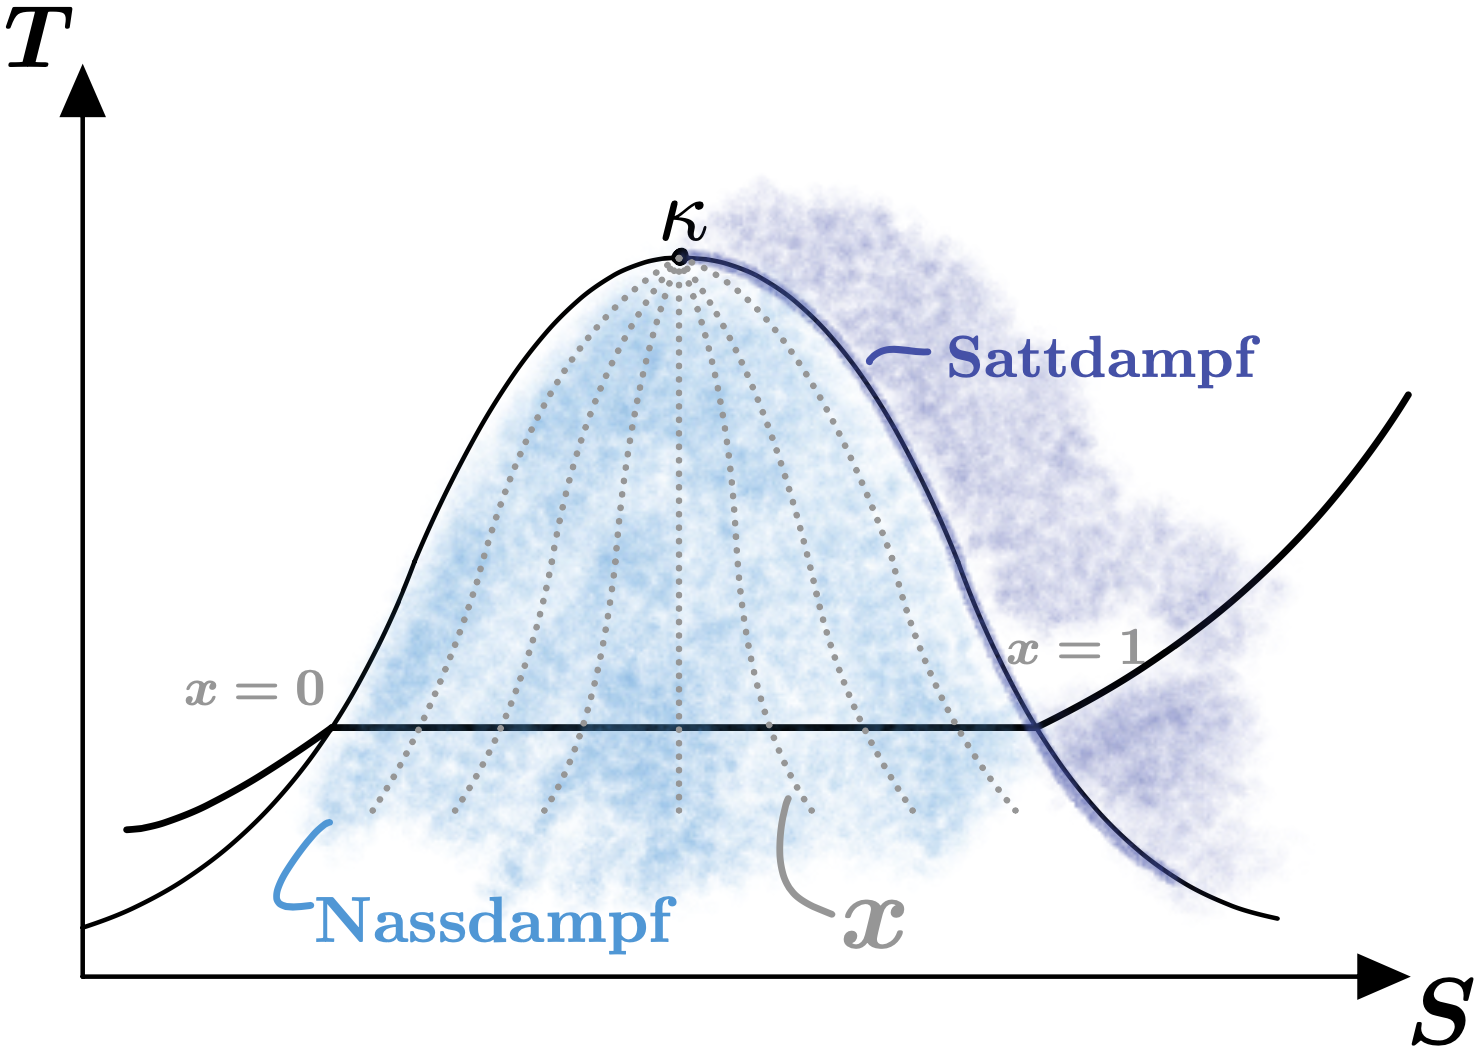
\includegraphics[width=4cm]{4-5_Nassdampfkurve}
\begin{itemize}[leftmargin=*]
        \item [] $h(x)=h'+x\cdot(h''-h')=h'+x\cdot r$
        \item [] $v(x)=v'+x\cdot(v''-v')$
        \item [] $s(x)=s'+x\cdot(s''-s')$
        \item [] unter der Nassdampfkurve gilt \textbf{nicht} $h_{12}=c_p\cdot (T_2-T_1))$
\end{itemize}

\columnbreak
%---------------------------------------------------------------------------

\subsubsection{Kreisprozesse Skizzen}
\begin{itemize}[leftmargin=*]
        \item [] \textbf{Dampfprozess:} (beispielhaft)\\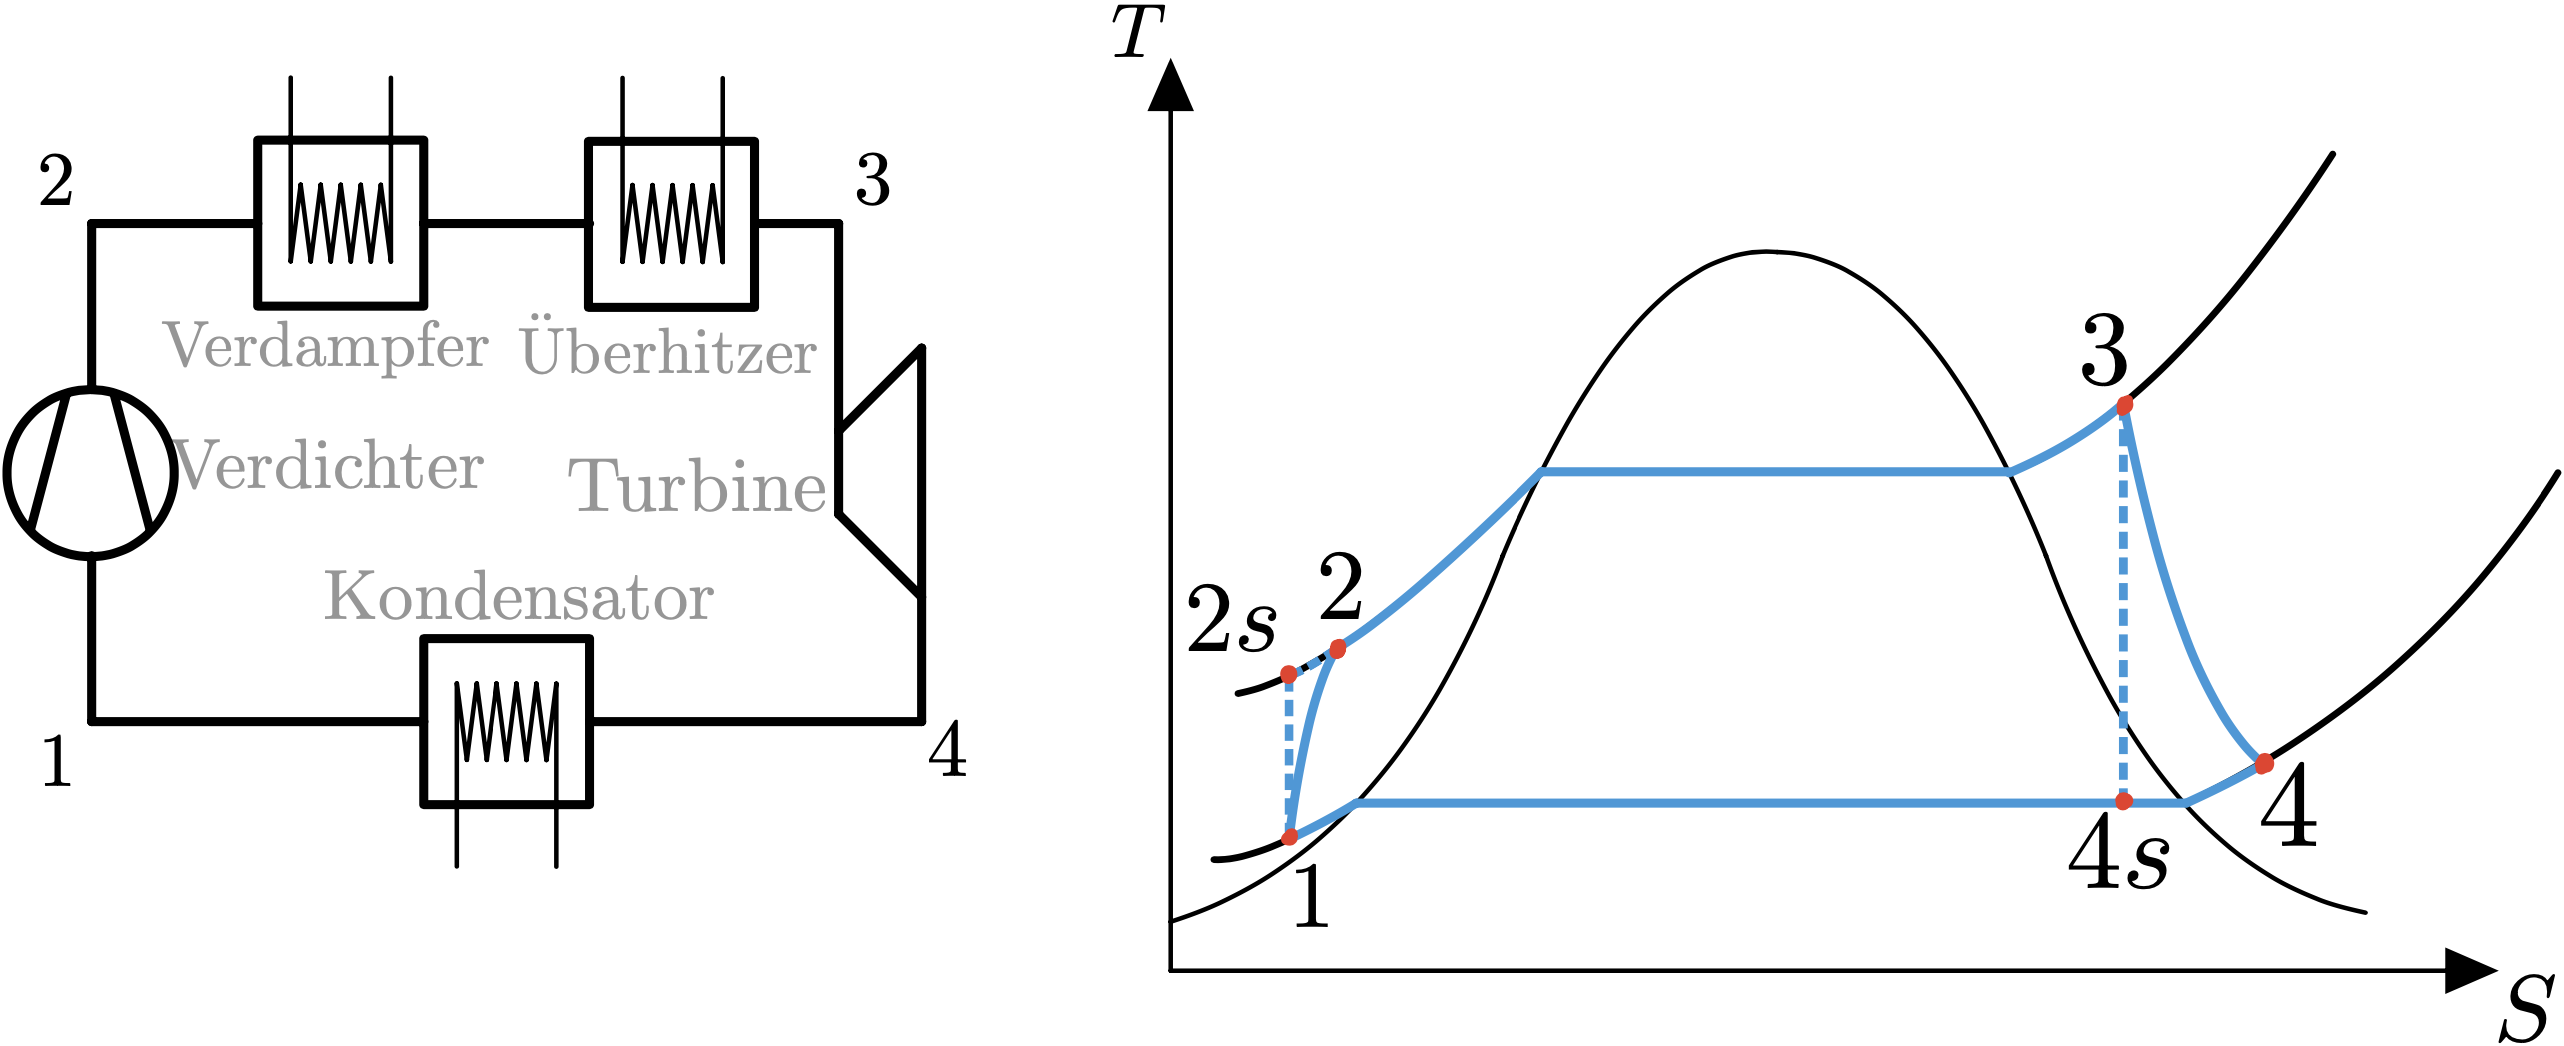
\includegraphics[width=8cm]{4-6-1_Dampfprozess}
        \item [] \textbf{Kälteprozess:} (beispielhaft)\\\includegraphics[width=8cm]{4-6-1_Kälteprozess}
        \item [] \textbf{Joule-Prozess:}\\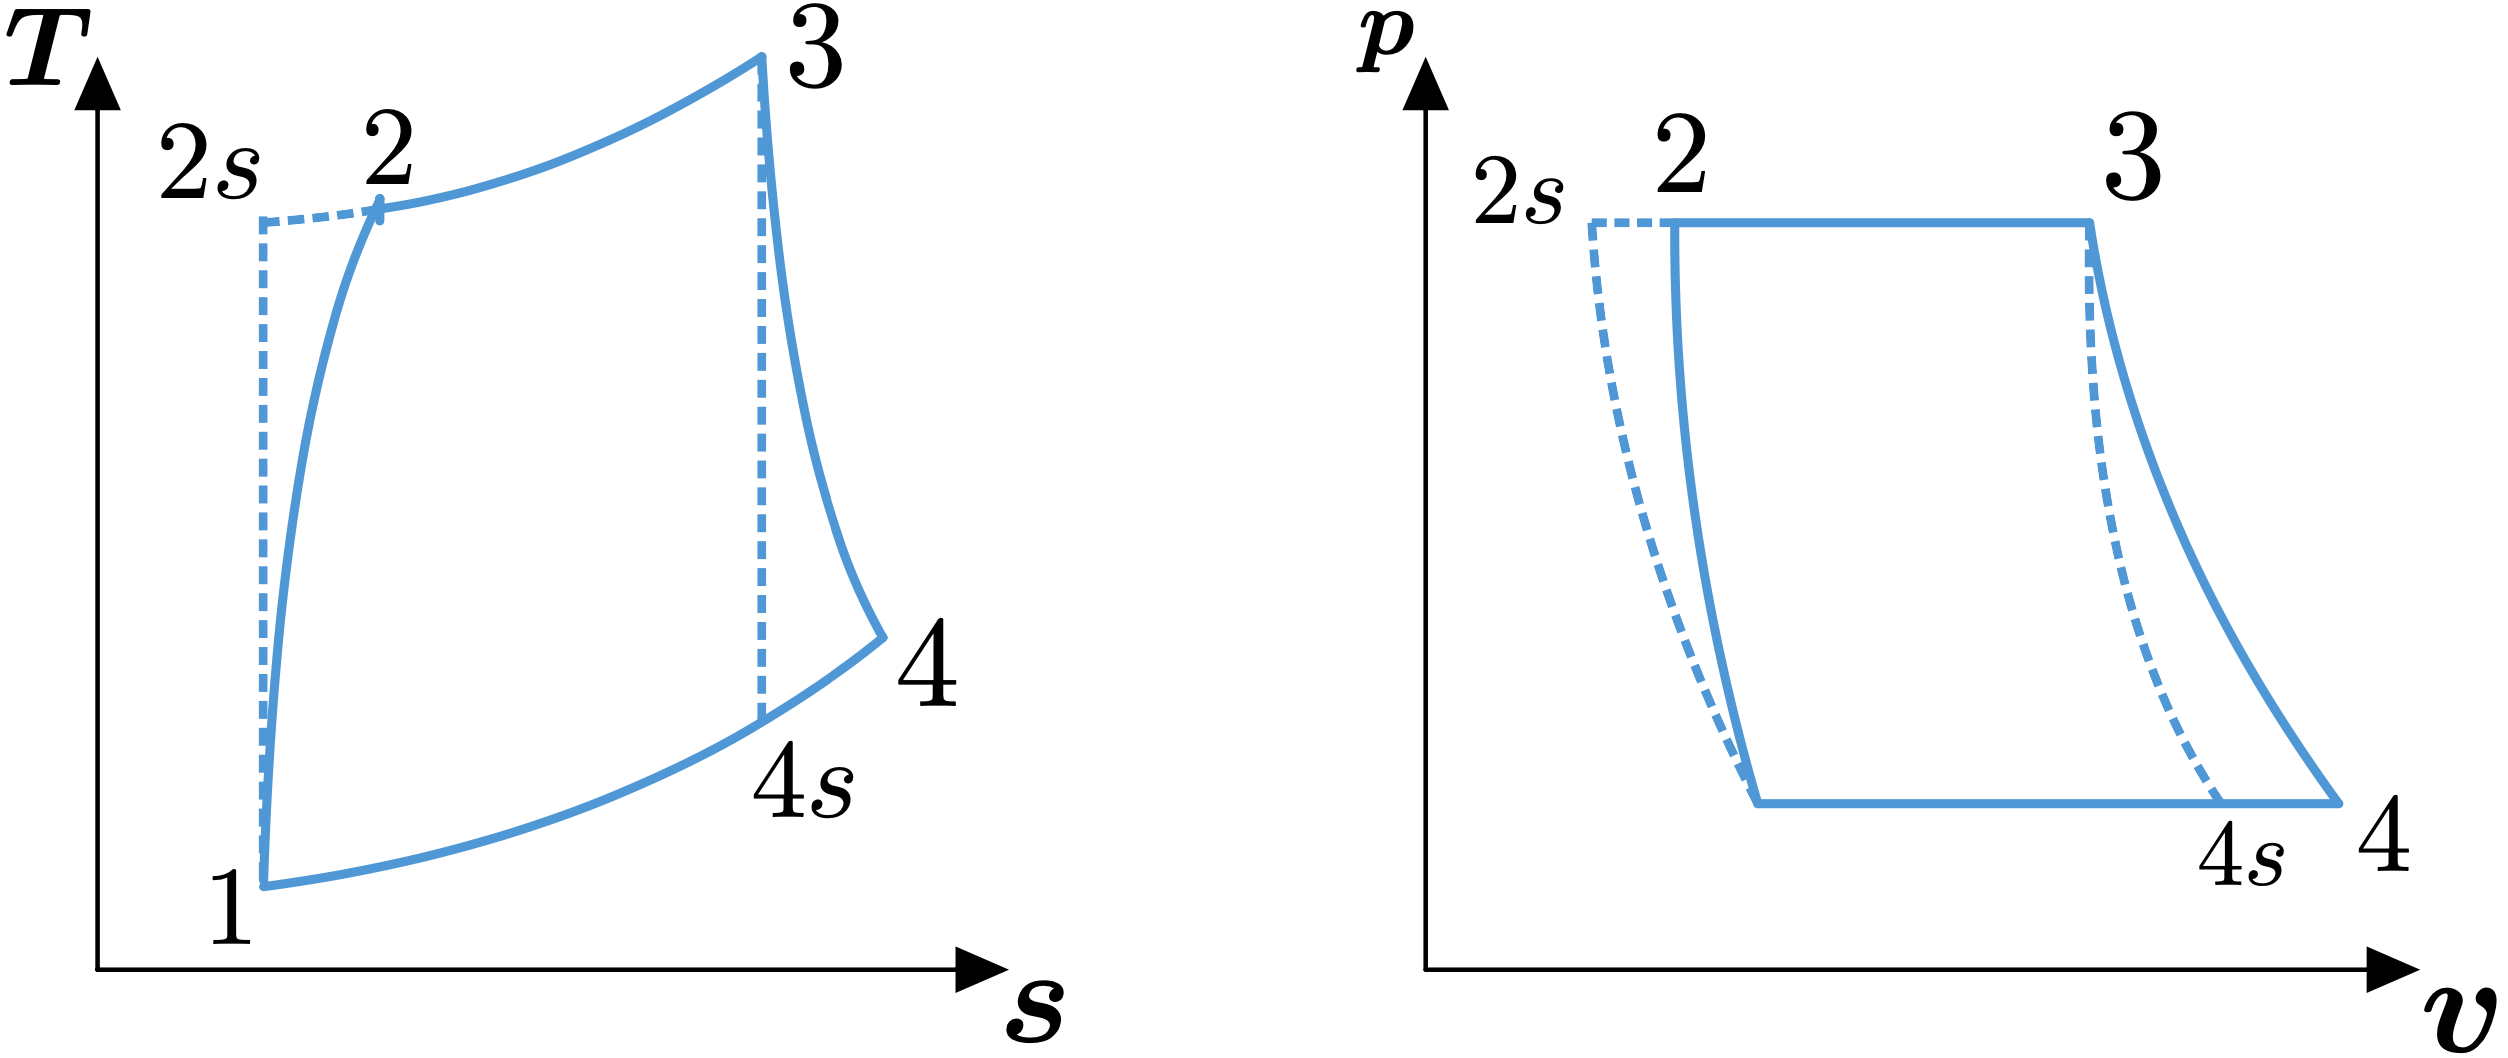
\includegraphics[width=6cm]{4-6-1_Joule-Prozess}
\end{itemize}

\subsection{Schmelzen}
%[!]TODO: Formel wahrscheinlich nicht richtig:
%[!]TODO: Biler/Diagramm einfügen
\begin{itemize}[leftmargin=*]
        \item [] $m_i\cdot c_i\cdot\Delta{T}+m_i\cdot q_s+m_i\cdot c_s\cdot T_M=m_s\cdot c_s\cdot(T_s-T_K)$
\end{itemize}

\section{Kinematik}
\subsection{Grundgleichungen}
\begin{itemize}[leftmargin=*]
        \item [] $s(t)=s_0+v_0\cdot t+\frac{a}{2}\cdot t^2$\tabto{4cm}$\phi(t)=\phi_0+\omega_0\cdot t+\frac{\alpha}{2}\cdot t^2$
        \item [] $v(t)=v_0+a\cdot t$\tabto{4cm}$\omega(t)=\omega_0+\alpha\cdot t$
        \item [] $v(s)=\sqrt{v_0^2+2\cdot a\cdot(s-s_0)}$
        \item [] $s=r\cdot\phi$\tabto{2cm}$v=r\cdot\omega$\tabto{4cm}$a=r\cdot\alpha$
\end{itemize}

\subsection{Geschwindigkeiten und Beschleunigungen bei Drehbewegungen}
\begin{itemize}[leftmargin=*]
        \item [] $v_r=\dot{r}$\tabto{2cm}$a_r=\ddot{r}-r\cdot\dot{\phi}^2$
        \item [] $v_t=r\cdot\dot{\phi}$\tabto{2cm}$a_t=r\cdot\ddot{\phi}+2\cdot\dot{r}\cdot\dot{\phi}$
\end{itemize}

\subsection{Absolutgeschwindigkeit \& Absolutbeschleunigung}
\begin{itemize}[leftmargin=*]
        \item [] $\vec{v_B}=\vec{v_A}+\vec{v_{AB}}$
        \item [] $\vec{a_B}=\vec{a_A}+\vec{a_{AB}}$
\end{itemize}

\columnbreak
%---------------------------------------------------------------------------

\section{Kinetik}
\subsection{Dynamik}
\begin{itemize}[leftmargin=*]
        \item [] \textbf{Impulssatz:} \tabto{2.3cm}$m\cdot\ddot{x}=\sum{F}$
        \item [] \textbf{Drallsatz:} \tabto{2.3cm}$J\cdot\ddot{\phi}=\sum{M}$
        \item [] \textbf{wichtige Kräfte:} \tabto{2.3cm}$F_\text{Feder}=c\cdot x_\text{F}\qquad F_\text{Dämpfer}=k\cdot\dot{x_\text{D}}$
        \item [] \textbf{wichtige Massenträgheitsmomente:}\\$J_\text{Zylinder}^S=\frac{m\cdot r^2}{2}\qquad J_\text{Kugel}^S=\frac{2}{5}\cdot m\cdot r^2\qquad J_\text{Stab}^S=\frac{m\cdot l^2}{12}$
        \item [] \textbf{Satz von Steiner:} \tabto{2.3cm}$J^P=J^S+m\cdot r^2$
\end{itemize}

\subsection{Energie \& Arbeit}
\begin{itemize}[leftmargin=*]
        \item [] $E_1+W_{zu}-W_{ab}=E_2$
        \item [] $W=\int{F\cdot ds}=\int{M\cdot d\phi}$
        \item [] \textbf{potentielle Energie:}\\$E_\text{pot}=W_\text{pot}=m\cdot g\cdot h$
        \item [] \textbf{kinetische Energie:}\\$E_\text{transl}=W_\text{transl}=\frac{m\cdot v^2}{2}\qquad E_\text{rot}=W_\text{rot}=\frac{J\cdot\omega^2}{2}$
        \item [] \textbf{Federenergie:}\\$E_\text{el}=W_\text{el}=\frac{c\cdot(s_1^2-s_2^2)}{2}=\frac{c\cdot(\phi_1^2-\phi_2^2)}{2}$
        \item [] \textbf{Reibungsenergie:}\\$E_\text{reib}=W_\text{reib}=F_N\cdot\mu\cdot s$
        \item [] \textbf{Massenreduktion:}\\$m_{red}\cdot\frac{v_{red}^2}{2}=J_{red}\cdot\frac{\omega_{red}^2}{2}=\sum{E_\text{kin}}$
        \item [] \textbf{Leistung:}\\$P=F\cdot v=M\cdot\omega=\frac{F\cdot s}{t}$
\end{itemize}

\subsection{Impuls \& Stoß}
\textbf{Impulserhaltung:}\tabto{3cm}$m_1\cdot\vec{v_1}=m_2\cdot\vec{v_2}=\text{konst.}$\\
\textbf{Stoß:}
\begin{itemize}[leftmargin=*]
        \item [] $u=\frac{m_{1\text{red}}\cdot v_1+m_{2\text{red}}\cdot v_2}{m_{1\text{red}}+m_{2\text{red}}}$
        \item [] $s_{K1}=m_1\cdot(u-v_1)\qquad s_{R1}=m_1\cdot(v_1'-u)$
        \item [] $s_{K2}=m_2\cdot(u-v_2)\qquad s_{R2}=m_2\cdot(v_2'-u)$
        \item [] $k=\frac{s_{R1}}{s_{K1}}=\frac{s_{R2}}{s_{K2}}=\frac{u-v_1'}{v_1-u}=\frac{v_2'-u}{u-v_2}\quad\longrightarrow\quad v_i'=(1+k)\cdot u-v_i\cdot k$\\ \\
        \subitem {\scriptsize $v_i$\tabto{1cm}...Geschwindigkeit von Masse $i$ vor dem Stoß}
        \subitem {\scriptsize $v_i'$\tabto{1cm}...Geschwindigkeit von Masse $i$ nach dem Stoß}
        \subitem {\scriptsize $u$\tabto{1cm}...gemeinsame Geschwindigkeit während der Kompressionsphase}
        \item [] $E_\text{kin0}+E_\text{pot0}-E_v=E_\text{kin1}+E_\text{pot1}\qquad\qquad E_v$ ...Verformungsenergie
\end{itemize}

\columnbreak

\subsection{Schwingungen}
\textbf{freie ungedämpfte Schwingung}
\begin{itemize}[leftmargin=*]
        \item [] $\ddot{\variant{x}}+\omega^2\cdot\variant{x}=0\qquad\qquad m\cdot\ddot{\variant{x}}+c\cdot\variant{x}=0$
        \item [] $\variant{x}(t)=A\cdot\sin(\omega\cdot t)+B\cdot\cos(\omega\cdot t)\qquad$bzw.$\qquad\variant{x}(t)=C\cdot\sin(\omega\cdot t+\psi)$
        \item [] $\quad\longrightarrow\quad A$ \& $B\quad\Leftarrow\quad$ aus Randbedingungen ermitteln
        \item [] $\quad\longrightarrow\quad C=\sqrt{A^2+B^2}$
        \item [] $\quad\longrightarrow\quad\psi=\arctan\left(\frac{A}{B}\right)$
\end{itemize}

\vspace{20pt}

\textbf{freie gedämpfte Schwingung}
\begin{itemize}[leftmargin=*]
        \item [] $\ddot{\variant{x}}+2\delta\cdot\dot{\variant{x}}+\omega^2\cdot\variant{x}=0$
        \item [] schwache Dämpfung: \fbox{$\delta^2<\omega^2$}
        \subitem $\variant{x}(t)=e^{-\delta\cdot t}\cdot\left( A\cdot\sin(\omega_d\cdot t)+B\cdot\cos(\omega_d\cdot t)\right)$
        \subitem \tabto{1.8cm}bzw.
        \subitem $\variant{x}(t)=C\cdot e^{-\delta\cdot t}\cdot\sin(\omega_d\cdot t+\psi)$
        \subitem $\quad\longrightarrow\quad\omega_d=\sqrt{\omega^2-\delta^2}$
        \subitem $\quad\longrightarrow\quad A$ \& $B\quad\Leftarrow\quad$ aus Randbedingungen ermitteln
        \subitem $\quad\longrightarrow\quad C=\sqrt{A^2+B^2}$
        \subitem $\quad\longrightarrow\quad\psi=\arctan\left(\frac{A}{B}\right)$
        \item [] starke Dämpfung: \fbox{$\delta^2>\omega^2$}
        \subitem $\variant{x}(t)=e^{-\delta\cdot t}\cdot\left(A\cdot e^{\sqrt{\delta^2-\omega^2}\cdot t}+B\cdot e^{\sqrt{\delta^2-\omega^2}\cdot t}\right)$
        \item [] aperiodischer Grenzfall: \fbox{$\delta^2=\omega^2$}
        \subitem $\variant{x}(t)=e^{-\delta\cdot t}\cdot(A+B\cdot t)$
\end{itemize}

\par\vspace{150pt}\null
\columnbreak
%---------------------------------------------------------------------------

\textbf{erzwungene Schwingung}
\begin{itemize}[leftmargin=*]
        \item [] $\ddot{\variant{x}}+2\delta\cdot\dot{\variant{x}}+\omega^2\cdot\variant{x}=A_e\cdot\sin(\Omega\cdot t)$\tabto{5.1cm}oder$\quad\dots=A_e\cdot\cos(\Omega\cdot t)$
        \item [] $x_p(t)=C\cdot\sin(\Omega\cdot t+\psi)$\tabto{5.1cm}oder$\quad\dots=C\cdot\cos(\Omega\cdot t+\psi)$
        \item [] $\quad\longrightarrow\quad A=\frac{A_e}{\sqrt{(\omega^2-\Omega^2)^2+4\cdot\delta^2\cdot\Omega^2}}$
        \item [] $\quad\longrightarrow\quad\psi=\arctan(\frac{2\cdot\delta\cdot\Omega}{\omega^2-\Omega^2})\qquad$ für $\psi<0$: $\quad\psi_{neu}=\psi+\pi$
        \item [] \vspace{7pt}{\scriptsize$\omega_\text{max}=\sqrt{\omega^2-2\delta^2}$}
        \item [] {\scriptsize wenn $\omega_\text{max}=\Omega\quad\rightarrow\quad$Resonanz}
\end{itemize}

\vspace{20pt}

\textbf{Federschaltungen}
\begin{itemize}[leftmargin=*]
        \item [] $c_\text{ers,parallel}=\sum_{i}^{n}c_i=c_1+c_2+\cdots$
        \item [] $c_\text{ers,seriell}=\frac{1}{\sum_{i}^{n}\frac{1}{c_i}}=\frac{1}{\frac{1}{c_1}+\frac{1}{c_2}+\cdots}$
\end{itemize}

\par\vfill\null
\columnbreak
%---------------------------------------------------------------------------

 
\vfill


\tabto{6.3cm}\rule{0.3\linewidth}{0.25pt}\\
\tiny
\tabto{6.3cm}\href{http://wch.github.io/latexsheet/}{http://wch.github.io/latexsheet/}\\
\tabto{6.3cm}Copyright \copyright\ 2014 Winston Chang\\
\tabto{6.3cm}Copyright \copyright\ \the\year\ Tobias Mittermair
\begin{flushright}
        {\normalsize V1.4}\\
\end{flushright}


\end{multicols*}
\end{document}
